\documentclass[11pt]{article}
\usepackage{cth_course_template}
\usepackage{times}
\usepackage{url}
\usepackage{latexsym}
\usepackage{graphicx}
\usepackage{caption}
\usepackage{subcaption}
\usepackage{cleveref}
\usepackage{hyperref}
\usepackage{siunitx}
\usepackage{csquotes}

\aclfinalcopy % Uncomment this line for the final submission
%\def\aclpaperid{***} %  Enter the acl Paper ID here

\title{Sentiment Analysis of Customer Reviews}

\author{Celio Bueri \\
  {\tt celio.bueri@gmail.com} \\\And
  Christoph Stelz \\
  CID \textttt{stelz} \\
  {\tt mail@ch-st.de} \\}

\date{April 2023}

\begin{document}
\maketitle
\begin{abstract}
We present multiple classifiers that distinguish positive from negative customer reviews based on text alone. To further improve classifier accuracy, we use triple-annotated training datasets and hyperparameter tuning with a grid search. Our best linear model is able to reach $96.7\%$ accuracy on an unseen test dataset and a fine-tuned Transformer-based model reaches even $98.6\%$.
\end{abstract}



\section{Introduction}
Our goal is to create a software that can automatically classify the customer reviews left on the Birch website according to whether they are positive (the customer is happy with his visit) or negative (bad customer experience).

This would improve the analytical abilities of  Birch Inc. to react to customer data.

\section{Method}

We use Keras~\cite{chollet2015keras} for the Transformer models and the scikit-learn package~\cite{scikit-learn} for all other machine learning algorithms.

\subsection{Training data preparation}
In a group effort, we first collected around $8\,769$ customer reviews.
We manually classified these reviews into 2 classes: positive and negative.
To prevent erroneous training labels, the reviews were labeled by several people.


While gathering an overview over the training dataset, we noticed that the annotators did not always agree.
We thought of three approaches on how to deal with the cases where several reviewers have rated the same review differently:

\begin{enumerate}
    \item create a third class "indeterminate" or "neutral" which contains both the review which are neither positive nor negative as well as the opinions where the annotators do not agree
    \item simply remove these cases from the training base
    \item manually resolve annotation disagreement by going over the dataset 
\end{enumerate}

We decided against approach 1 because entries with unequal annotations are not necessarily representative of neutral reviews and introducing such a label might produce misleading results.

Furthermore, after looking at the number of these indeterminate cases and finding that only 396 reviews (around $5.64\%$ of our data) are affected, we deemed that removing them from the set is tolerable.
Thus, we went with approach 2.

Apart from the training set, we were also provided with a test dataset containing around $1\,751$ reviews.
This was kept aside until the very end.
We split off around one third of the training dataset to be used for validation of our classifiers during tuning.

\subsection{Extended training data preparation}
A second training dataset was triple-annotated by three different reviewers.
Again, some rows were incorrectly labeled.
To resolve unequal annotations, we performed a majority vote: at least two labels must be “positive” or “negative” for the review to be considered “positive“ or “negative”, respectively.
If two or more annotations were invalid, we simply discarded the rows.
This was only the case for 100 rows, meaning $98.7\%$ of the extended training dataset could be used.

\subsection{Feature extraction}

Because there was no metadata supplied about the reviews, the only data we have to classify them is the text of the reviews themselves.
Since most classification algorithms work on numerical inputs, we need a way to turn the review character string into a passable input for other classifiers.

One approach is treating the review text as an unordered list of words (\textbf{bag of words} representation). It is the presence and number of occurrences of certain words that allows us to classify the review.
A \texttt{CountVectorizer} normalizes the string and turns it into a sparse vector, were each word or n-gram is a single entry of the vector set to the number of occurrences.
To alleviate the influence of the review length on the feature vectors, a \texttt{TfidfTransformer} is employed. It uses the weighting expression $\textrm{term frequency} / \textrm{document frequency}$.

Another approach is the \textbf{Word2Vec} approach~\cite{mikolov_efficient_2013}.
It uses a shallow neural network to generate vectors from words.
This allows the vectors to carry some meaning of the vocabulary, for example the distance from ``red'' to ``blue'' should be shorter than ``red'' to ``sky''.
During preliminary tests with Word2Vec pretrained on the Google News 300 dataset, the classification was much worse than with a \texttt{TfidfTransformer}.
Due to time constraints, we therefore deemed this approach unfeasible and decided to focus on the first approach.

A third approach is the Transformer model underlying the BERT language model~\cite{devlin2018bert}.
This model is pre-trained on an enormous corpus of text and learns to weight the significance of input tokens during this process.
In contrast to the \texttt{TfidfTransformer}, the Transformer model also uses Positional Encoding~\cite{vaswani_attention_nodate} such that the placement of words relative to each other can be taken into account by the actual classifier. This provides a substantial benefit: for example, a reviewer could “have visited worse places”. In this case, the bag of word representation can not discern that the negative word \textit{worse} is referencing a past event not related to the current restaurant.


\subsection{Classifiers}
Aside from the Neural-Network-based Transformers, we chose three linear classifiers: Gradient Boosted Decision Trees (GBC), Support Vector Classifier (SVC) and a simple Logistic Regression.
We chose SVC in particular because our input data is high-dimensional. The \texttt{TfidfTransfomer} extracts around $9\,239$ features from the input text.
Logistic Regression was chosen as a simple baseline method to compare against the more complicated models.

At first, we trained all classifiers using the default hyperparameters of scikit-learn.
We then focused on the SVC, because its validation accuracy looked very promising (see \Cref{sec:hypertuning} for details.).

A big advantage of the linear models is their interpretability.
Therefore, as a sanity check, we can then use the weights associated with the features to see which words express the most positive or negative opinions.
 (A large positive coefficient expresses that this word gives a positive opinion, a big negative coefficient shows a
 negative opinion and a word with an almost null coefficient is neutral concerning the opinion).
 As can be seen in the two word clouds of \Cref{fig:wordcloud}, the results are quite intuitive. Words like “delicious”, “excellent” and “amazing” are indicators for a positive review, while “slow”, “horrible” and “bland” are more likely to occur in a negative review.

 \begin{figure}
     \centering
     \begin{subfigure}[b]{1\linewidth}
         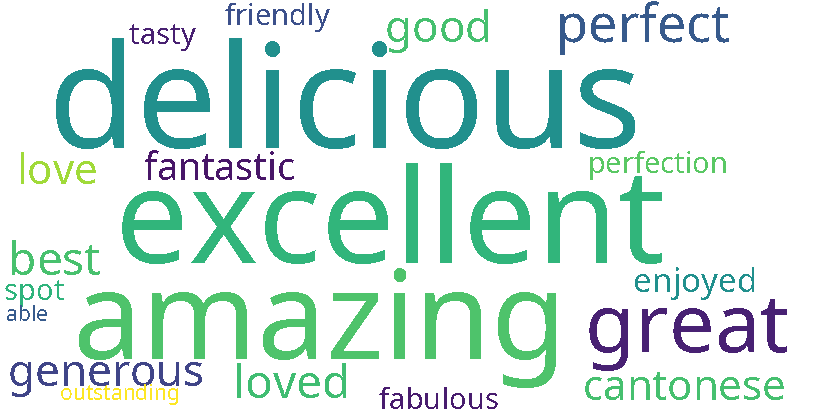
\includegraphics[width=1\linewidth]{figures/wordcloud_positive.pdf}
         \caption{positive}
         \label{fig:wordcloud_pos}
     \end{subfigure}
     \begin{subfigure}[b]{1\linewidth}
         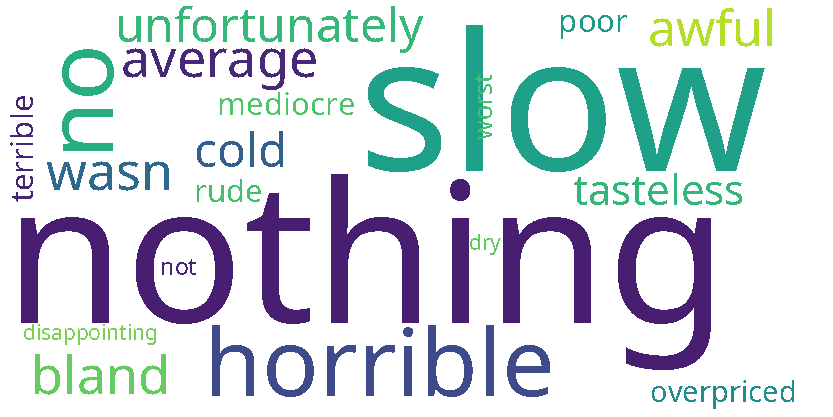
\includegraphics[width=1\linewidth]{figures/wordcloud_negative.pdf}
         \caption{negative}
         \label{fig:wordcloud_neg}
    \end{subfigure}
     \caption{Positively and negatively associated features learned by the SVC}
     \label{fig:wordcloud}
 \end{figure}



\subsection{Hyperparameter Tuning}
\label{sec:hypertuning}

To further improve the SVC, we decided to perform a grid search with step size $0.1$ on the regularization hyperparameter $C$.
As we can see in \Cref{fig:svc_acc}, increasing $C$ yields a better training accuracy until our classifier matches our training dataset almost perfectly.
However, the improvements in the accuracy on the validation set level off very quickly, and no improvements can be seen for $C > 1$.
This is a clear indicator that the model is overfitting for high values of $C$.
The best value for $C$ found by our grid search is $1.0$, which coincidentally is also the default value of scikit-learn.

\begin{figure}
    \centering
    %TODO: change label from test to validation
    
\includegraphics[width=0.85\columnwidth]{figures/svm_accuracy.pdf}
    \caption{Validation accuracy of the SVC for different regularization values}
    \label{fig:svc_acc}
\end{figure}

Another parameter we tried tuning is the n-gram size of our \texttt{CountVectorizer}. By default it is set to $1$, meaning monograms (single words) are considered for feature extraction. We tried setting it to the range $(1, 2)$, meaning both mono– and bigrams can be extracted from our input text. We simultaneously ran another grid search on $C$ and found that the best value for $C$ now was $1.2$.
However, the validation accuracy of our SVC had not improved.

\subsection{Language-models}

The BERT model comes in different variants:
\begin{itemize}
    \item \textit{tiny}~\cite{bhargava2021generalization}, which has $L=2$ layers and a hidden size of $H=128$
    \item \textit{base}~\cite{devlin2018bert} with $L=12$ and $H=768$
\end{itemize}

The uncased (case-insensitive) pre-trained models were loaded with Keras and then fine-tuned on our dataset.
Fine-tuning was performed on Google Colab with a T4 GPU as accelerator.

The tiny variant was trained for 6 epochs. Because of resource limitations the base variant was only trained for 4 epochs.
\Cref{fig:bert_history} shows training and validation accuracy over the course of training the model.
The validation accuracy of the tiny variant does not improve much after 3 epochs and the base variant performs really good after only single epoch of training.
This goes to show the versatility of the Transformer model, their advantage being that they have already seen a large number of English text before we trained them on our review dataset.

\begin{figure}
    \centering
    \begin{subfigure}[b]{1\columnwidth}
    % todo: increase x axis by one.
        \centering
        
\includegraphics[width=0.85\columnwidth]{figures/bert_tiny_accuracy.pdf}
        \caption{tiny}
        \label{fig:bert_tiny}
    \end{subfigure}
    \begin{subfigure}[b]{1\columnwidth}
        \centering
        
\includegraphics[width=0.85\columnwidth]{figures/bert_base_accuracy.pdf}
        \caption{base}
        \label{fig:bert_base}
    \end{subfigure}
    \caption{Training history of BERT}
    \label{fig:bert_history}
\end{figure}

\section{Results}

\Cref{fig:final_accuracy} shows the accuracy of all classifiers on the never-before seen test dataset.
Rather unsurprisingly, the huge language model BERT base dominates, with a testing accuracy of $98.572\%$.
Interestingly, it does not improve from the triple-annotated dataset and even loses a bit of accuracy. This could be due to encoding issues (see \Cref{sec:limitations}).
In the category of linear models, SVC performs the best.
By tuning its hyperparameters and by training on the triple-annotated dataset, we were able to gain a whole percentage point in accuracy. Because SVC does not use a pretrained vectorizer like BERT, the encoding issues do not matter, and the larger training set size as well as the improved annotation quality\footnote{In the triple-annotated dataset, only $1.3\%$ of rows were removed instead of the $5.65\%$ from the original set, we consider this a rough proxy of annotation quality} allow it to improve its predictions.
SVC even outperforms the BERT tiny model, at a tiny fraction of the compute resources.

\begin{figure}
    \centering
    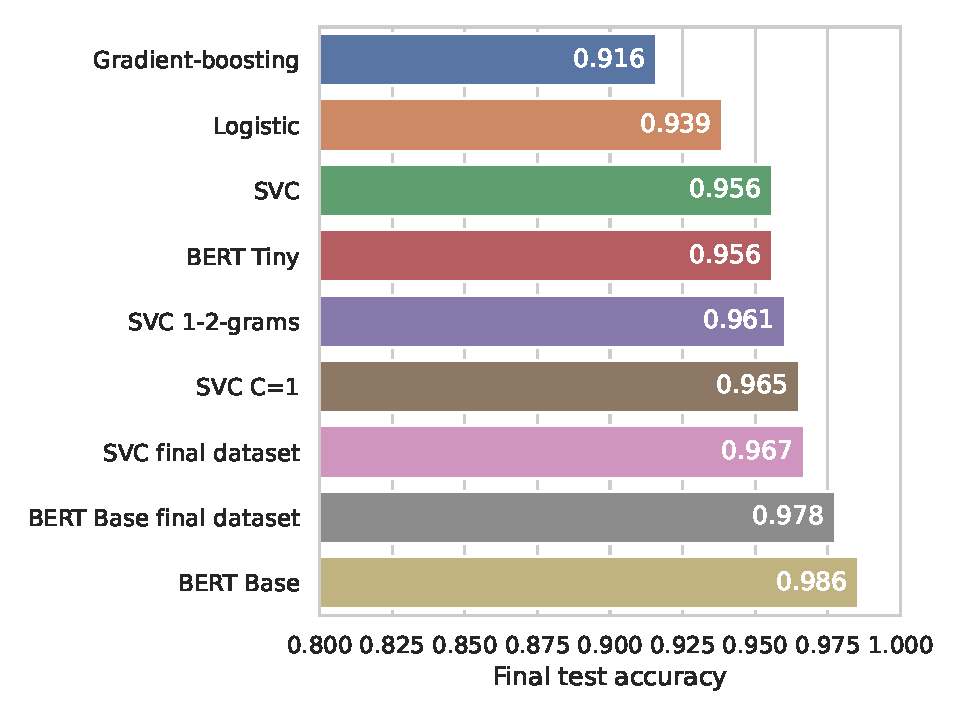
\includegraphics[width=\columnwidth]{figures/accuracy_barplot.pdf}
    \caption{Accuracy of the different classifiers}
    \label{fig:final_accuracy}
\end{figure}


\subsection{Performance}

For BERT tiny and base, the GPU-accelerated inference of a single review label took around \qty{1.21}{\milli\second} and \qty{5.30}{\milli\second} respectively.
The SVC was able to infer the labels on the CPU in less than \qty{40}{\micro\second}.

\subsection{Quality Control}
Aside from the accuracy scores being calculated on the unseen test dataset, we also spot checked the misclassified reviews to see if any pattern arises. The annotations seemed to be correct, so our training data was not at fault.

For BERT tiny, some of the misclassified reviews are ambivalent. For example, the service is praised but the food quality is lamented, or they speak highly of another restaurant. However, because of the small number of misclassifications (40), it is hard to say what went wrong exactly, especially because these large language models are not interpretable.

When calculating the confusion matrices, it is interesting that both SVC and the BERT classifiers produce more false negatives than false positives.
Again by spot-checking we built the theory that negations like \enquote{not bad}, \enquote{didn't care about} mislead our classifiers, but further factual research is necessary to confirm this hypothesis.

\section{Conclusion}

We presented two approaches to classifying the sentiment of customer reviews.
We were able to attain a near $99\%$ accuracy for an unseen test dataset.

Concerning the deployment of the classifiers, our recommendation is twofold:
\begin{enumerate}
    \item For high-throughput use cases, where a large number of reviews is classified, we recommend the SVC trained on the triple-annotated dataset. Its accuracy of $96.7\%$ ranks high and possible missclassifications would not matter when analyzing statistical measures like average or median. Furthermore, it is computationally inexpensive and can quickly work through large amounts of data.
    \item For delicate analysis of singular review texts, we recommend the fine-tuned BERT base classifier. It has near $99\%$ accuracy and could be useful in situations where false-positives are undesirable, e.g. when a survey email should be sent out to a customer if he has left a bad review. Its downside is that it needs GPU acceleration to run at sufficient speeds, since CPU inference is slow. 
\end{enumerate}

\subsection{Limitations, Biases \& Outlook}
\label{sec:limitations}

Since the task given to our fellow students during the data collection phase was to find positive or negative reviews, ambivalent or neutral reviews are most likely not well represented.
Spot-checking our dataset confirms the existence of this bias.

Also, the triple-annotated training dataset contained encoding errors of special characters in a lot of reviews.
We only noticed this very late into the project and were unable to make corrections.
The \texttt{CountVectorizer} of the SVC is able to improve despite this, because the exact spelling of tokens does not matter to the feature extraction.
However, we believe that the BERT model could be improved beyond the $98.6\%$ mark with a corrected triple-annotated dataset.

\subsection{Reproducibility}
All of the source code used to train and test the classifiers, as well as the code for the plots is available in a GitHub repository\footnote{\url{https://github.com/stelzch/review_sentiment_analysis}}.
The repository also contains the weights for the fine-tuned BERT classifiers.
Training data is available on request; we chose not to publish it in the repository due to potential copyright violations.

\bibliographystyle{cth_course_template}
\bibliography{template}

\end{document}
